\chapter{Proposed approach and novelty}
\label{chap:approach}

This chapter defines the algorithmic starting point against which every
proposed modification in Chapter~\ref{chap:experiments} is measured. It
fixes, in detail, the exact baseline configuration, representation,
decoding procedure, and operators shared by the baseline and every
extension evaluated later, so that Chapter~\ref{chap:experiments}'s
comparisons isolate the effect of each proposed change rather than any
incidental difference in the surrounding machinery.

\section{Definition of the baseline algorithm}
\label{sec:baseline-definition}

The baseline used for comparison is the Genetic Programming Hyper-Heuristic
(GPHH) method for MRCPSP introduced by Tian, Mei, and Zhang~\cite{Tian2024GPHH},
presented at the 2024 IEEE Congress on Evolutionary Computation. \changed{The
authors' own implementation, available at
\url{https://github.com/TianYuanSX/GP\_MRCPSP\_CEC2024}, is used unmodified
as the baseline throughout this thesis. The following subsections describe
its components in turn: the core idea, the individual representation and
its terminal sets, the schedule construction procedure, the fitness
evaluation, and the evolutionary operators and parameters.} GPHH is
evaluated on the same MMLIB50 and MMLIB100 benchmark sets as the proposed
algorithm, making it a directly comparable starting point.

\subsection{Core idea: evolving heuristics rather than schedules}

GPHH belongs to the class of hyper-heuristic methods: instead of searching for good schedules directly, it uses Genetic Programming to automatically evolve scheduling priority rules.
Each evolved rule is an executable symbolic expression that, when applied inside a Schedule Generation Scheme (SGS), determines which activity to schedule next and in which execution mode.
The GP search operates at the level of rules, not solutions; once the best rule has been found on a training set of instances, it is applied to new instances without any further search.
\changed{Figure~\ref{fig:gphh-architecture} gives an overview of the whole pipeline; the remaining subsections describe its stages in turn.}

\begin{figure}[t]
  \centering
  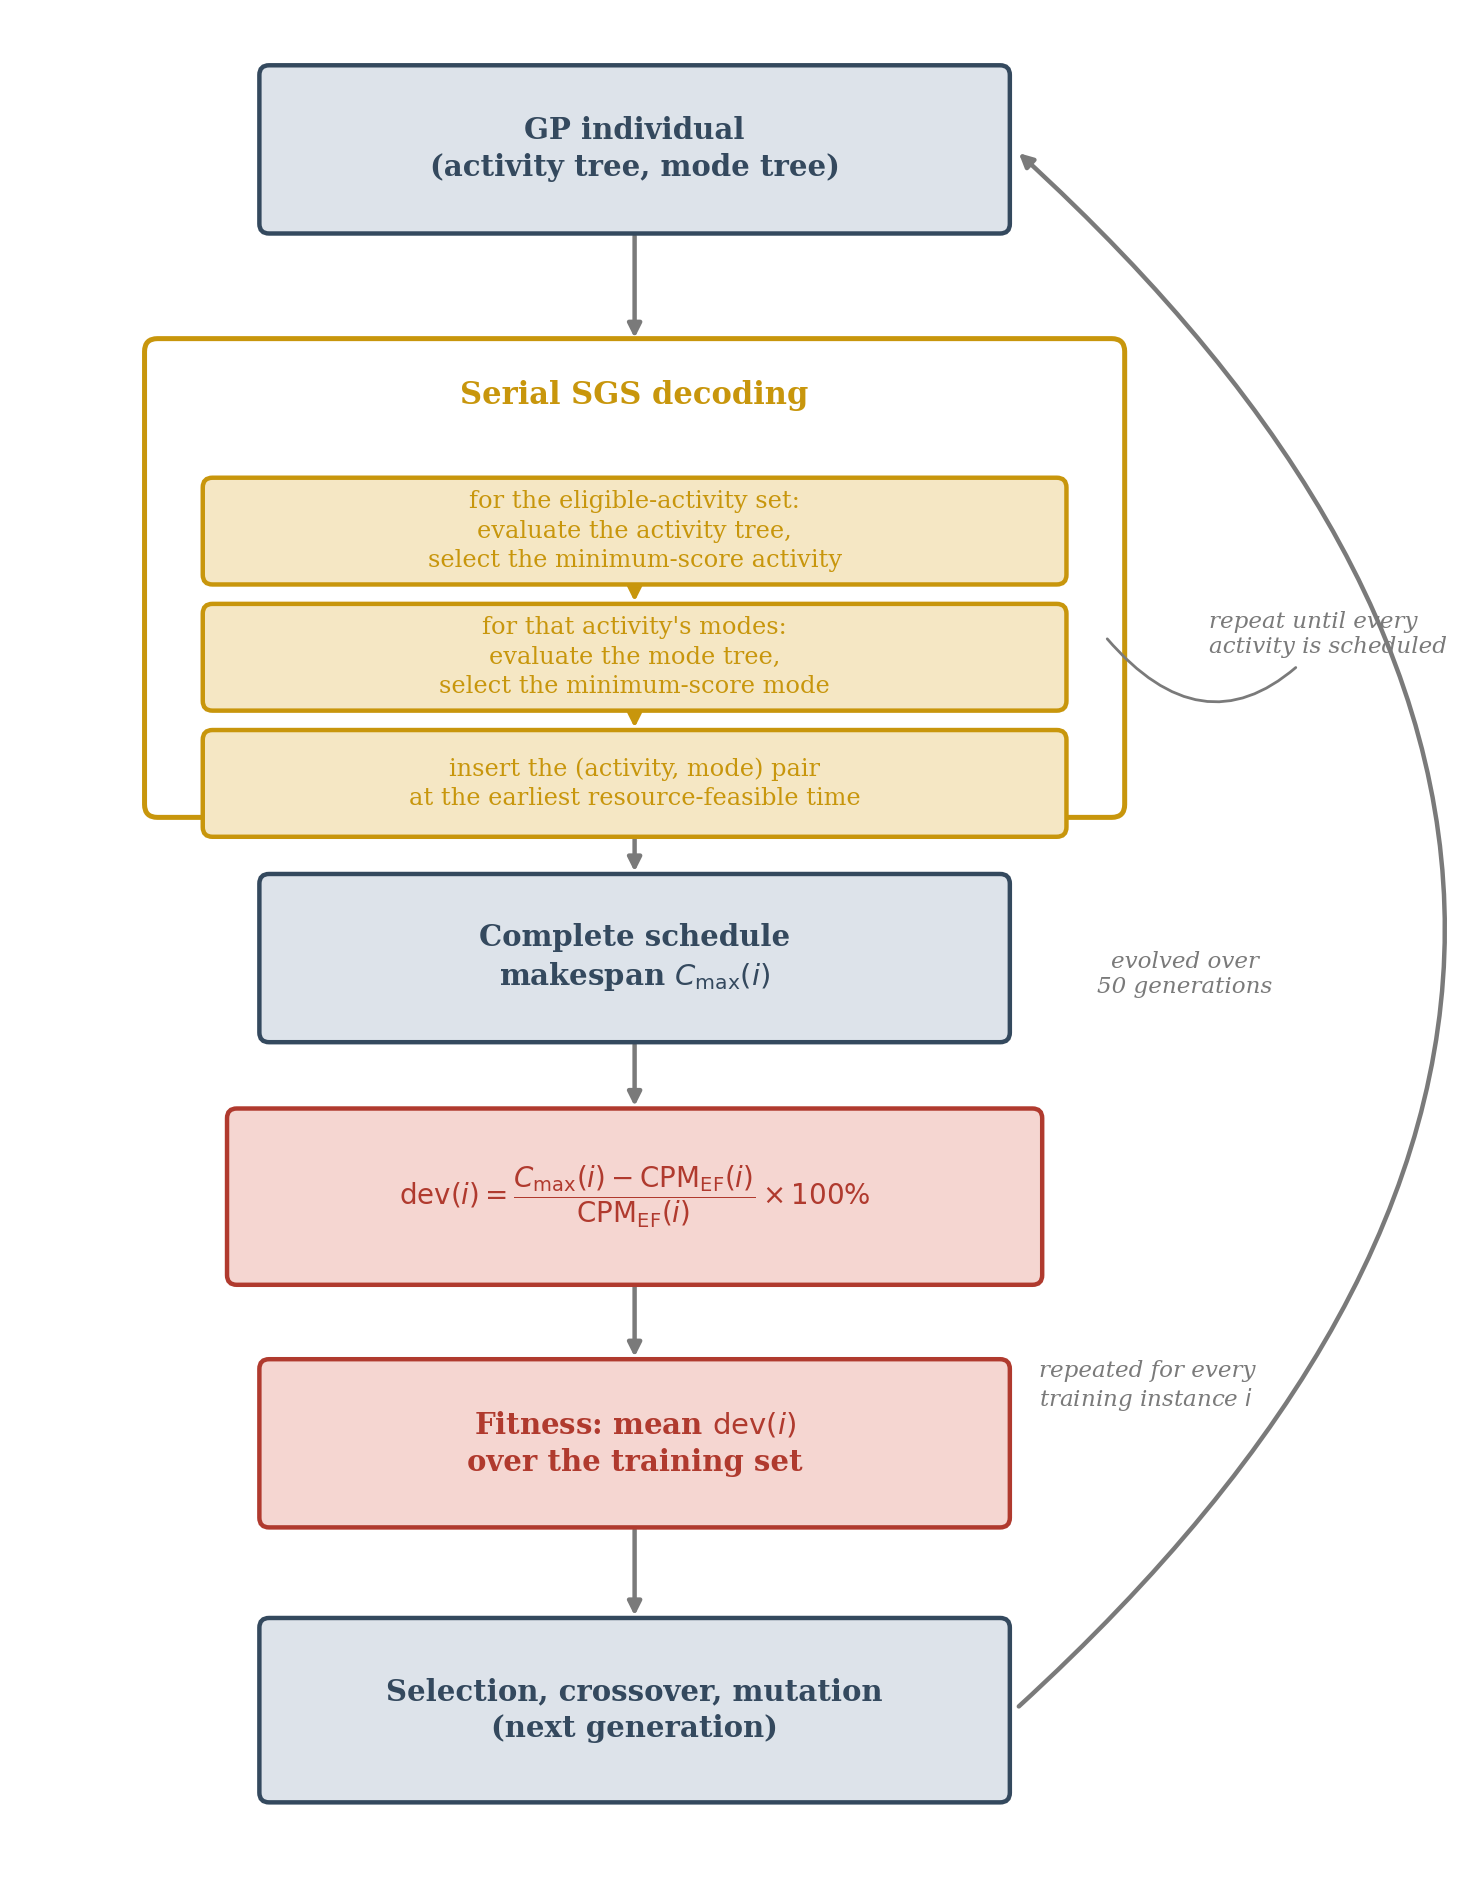
\includegraphics[width=0.78\textwidth]{img/gphh-architecture.png}
  \caption[The baseline GPHH pipeline]{Overview of the baseline GPHH
  pipeline: a multi-tree individual drives the serial SGS decoding loop to
  produce a complete schedule, whose deviation from the CPM lower bound is
  averaged over the training set to obtain the individual's fitness, which
  in turn drives selection, crossover and mutation for the next generation.
  The remaining subsections of this section detail each stage.}
  \label{fig:gphh-architecture}
\end{figure}

\subsection{Individual representation: multi-tree GP}
\label{subsec:individual-representation}

Each individual in the GP population is a pair of symbolic expression trees evolved simultaneously.
The \emph{activity tree} computes a numeric priority value for each eligible activity; the activity with the lowest value is selected next.
The \emph{mode tree} then computes a priority value for each available execution mode of the selected activity; again the mode with the lowest value is assigned.
This two-tree structure (referred to as \texttt{activity\_first} in the implementation) separates the activity-selection and mode-selection decisions into independently evolved sub-rules.

Both trees are constructed from a shared \textbf{function set}: \texttt{add}, \texttt{sub}, \texttt{mul}, \texttt{div} (protected against division by zero), \texttt{min}, and \texttt{max}.
The \textbf{terminal sets} differ between the two trees to reflect the information relevant at each decision stage\changed{, and are defined precisely in Tables~\ref{tab:activity-terminals} and~\ref{tab:mode-terminals}.
In the definitions, $j$ denotes the candidate activity, $\mathcal{M}_j$ its set of modes, $d_{jm}$ the duration of mode $m$, $\mathcal{K}$ the set of resource types, $r_{jmk}$ the requirement of mode $m$ for resource $k \in \mathcal{K}$, and $d^{\min}_j = \min_{m \in \mathcal{M}_j} d_{jm}$ the shortest duration available to activity $j$; $P_j$ and $S_j$ are the sets of immediate predecessors and successors of $j$ (Section~\ref{subsec:passes}), and $\bar{P}_j$ and $\bar{S}_j$ the corresponding transitive closures (all direct and indirect predecessors and successors).
The activity-tree terminals are static: they are computed once per instance, before decoding starts, with the four CPM dates obtained from one forward and backward pass (Section~\ref{subsec:passes}) on the resource-relaxed instance with every activity at its shortest duration $d^{\min}_j$.
Of the mode-tree terminals, only EFFT is dynamic, i.e.\ depends on the state of the partially built schedule at the moment the rule is queried; the remaining terminals are properties of the candidate mode or of the instance.}

\changedC{The order just described, select the activity first, then its
mode, is only one way to organise the decision, and Tian et
al.~\cite{Tian2024GPHH} define three variants, called \emph{GP decision
strategies} throughout this thesis; every experiment of
Chapter~\ref{chap:experiments} is run under each of the three.
Under \emph{activity-first} (the variant described above), the activity
tree scores every eligible activity, the lowest-scoring activity is
selected, and the mode tree then scores only that activity's modes to pick
one. Under \emph{mode-first}, the order is reversed: the mode tree first
commits a mode for every eligible activity (each activity's
lowest-scoring mode), and the activity tree then chooses among the
eligible activities, each already seen in its committed mode; the chosen
activity is scheduled in that mode. Because the mode is fixed before the
activity decision, the mode-first activity tree drops the across-modes
aggregates of Table~\ref{tab:activity-terminals} (the
\texttt{avg/max/min\_task\_duration} and \texttt{RReq\_m} terminals),
which would be redundant in that context. Under \emph{simultaneous},
finally, the individual is a single integrated tree rather than a pair:
it draws on the combined terminal vocabulary of both tables and scores
every eligible (activity, mode) pair jointly, and the lowest-scoring pair
is scheduled. Activity-first and mode-first therefore both evolve two
coupled trees and differ in which decision constrains which, while
simultaneous evolves one rule over the joint decision space, a
distinction that Section~\ref{subsec:nr-eval} shows to matter.}

\begin{table}[htbp]
  \centering
  \caption[Terminal set of the activity tree]{\changed{Terminal set of the
  activity tree. All terminals are computed
  once per instance before decoding.}}
  \label{tab:activity-terminals}
  \small
  \begin{tabularx}{\textwidth}{@{}l X@{}}
    \toprule
    \textbf{Terminal} & \textbf{Definition} \\
    \midrule
    \texttt{PC} & $|P_j|$ \\
    \texttt{TPC} & $|\bar{P}_j|$ \\
    \texttt{SC} & $|S_j|$ \\
    \texttt{TSC} & $|\bar{S}_j|$ \\
    \texttt{GRPW} & $d^{\min}_j + \sum_{i \in S_j} d^{\min}_i$
      (Greatest Rank Positional Weight) \\
    \texttt{GRPW\_all} & $d^{\min}_j + \sum_{i \in \bar{S}_j} d^{\min}_i$ \\
    \texttt{ES}, \texttt{EF}, \texttt{LS}, \texttt{LF} & $EST_j$, $EFT_j$,
      $LST_j$, $LFT_j$ (Section~\ref{subsec:passes}),
      computed on the resource-relaxed instance with durations $d^{\min}_j$ \\
    \texttt{avg\_task\_duration} &
      $\frac{1}{|\mathcal{M}_j|} \sum_{m \in \mathcal{M}_j} d_{jm}$ \\
    \texttt{max/min\_task\_duration} &
      $\max_{m \in \mathcal{M}_j} d_{jm}$,\;
      $\min_{m \in \mathcal{M}_j} d_{jm}$ \\
    \texttt{avg\_RReq\_m} &
      $\frac{1}{|\mathcal{M}_j|\,|\mathcal{K}|}
       \sum_{m \in \mathcal{M}_j} \sum_{k \in \mathcal{K}} r_{jmk}$ \\
    \texttt{max/min\_RReq\_m} &
      $\max_{m \in \mathcal{M}_j,\, k \in \mathcal{K}} r_{jmk}$,\;
      $\min_{m \in \mathcal{M}_j,\, k \in \mathcal{K}} r_{jmk}$ \\
    \bottomrule
  \end{tabularx}
\end{table}

\begin{table}[t]
  \centering
  \caption[Terminal set of the mode tree]{\changed{Terminal set of the mode
  tree, evaluated for a candidate mode
  $m$ of the selected activity $j$. Only \texttt{EFFT} depends on the
  current decoding state.}}
  \label{tab:mode-terminals}
  \small
  \begin{tabularx}{\textwidth}{@{}l X@{}}
    \toprule
    \textbf{Terminal} & \textbf{Definition} \\
    \midrule
    \texttt{task\_duration} & $d_{jm}$ \\
    \texttt{EFFT} & $\mathrm{EFFT}_{jm} = \min_{t \in F_{jm}} (t + d_{jm})$,
      where $F_{jm}$ is the set of feasible start times of $j$ in mode $m$
      under the current partial schedule; the mode-selection rule of Lova,
      Tormos and Barber~\cite{lova2006mrcpsp} \\
    \texttt{RR} & $|\{\,k \in \mathcal{K} : r_{jmk} > 0\,\}|$ \\
    \texttt{GRD} & $d_{jm} \cdot |\{\,k \in \mathcal{K} : r_{jmk} > 0\,\}|$ \\
    \texttt{avg\_RReq} &
      $\frac{1}{|\mathcal{K}|} \sum_{k \in \mathcal{K}} r_{jmk}$ \\
    \texttt{max/min\_RReq} &
      $\max_{k \in \mathcal{K}} r_{jmk}$,\;
      $\min_{k \in \mathcal{K}} r_{jmk}$ \\
    \texttt{avg\_ResCap} &
      $\frac{1}{|\mathcal{K}|} \sum_{k \in \mathcal{K}} R_k$
      (instance constant; $R_k$ is resource $k$'s capacity) \\
    \texttt{max/min\_ResCap} &
      $\max_{k \in \mathcal{K}} R_k$,\;
      $\min_{k \in \mathcal{K}} R_k$ \\
    \bottomrule
  \end{tabularx}
\end{table}

\subsection{Schedule construction via SGS}
\label{subsec:sgs-construction}

\changedB{At runtime the evolved rule pair drives the serial SGS of
Algorithm~\ref{alg:serial-sgs} (Section~\ref{subsec:sgs}), with one
multi-mode extension.}
\changedB{The activity tree plays the role of the priority rule $\pi$: at
each step it is evaluated for every eligible activity (those whose
predecessors have all been completed) and the activity $j^{*}$ with the
minimum score is chosen. The selection of $j^{*}$ is followed by one extra
step that the single-mode statement of Algorithm~\ref{alg:serial-sgs} does
not need: the mode tree is evaluated for every available mode
$m \in \mathcal{M}_{j^{*}}$ and the mode with the minimum score is
assigned.}
The activity is inserted into the schedule at the earliest time at which all renewable resource requirements of the chosen mode are satisfied.
This process repeats until all activities are scheduled.

\subsection{Fitness evaluation}
\label{subsec:fitness-evaluation}

Each individual is evaluated on a fixed \emph{training set} of MRCPSP instances drawn from the MMLIB benchmark library.
\changed{The reference value for each instance is its \emph{CPM lower bound}
$\mathrm{CPM}_{\mathrm{EF}}(i)$: the critical-path length of instance $i$,
computed by one CPM pass (Section~\ref{subsec:passes}) with all resource
constraints relaxed and every activity at its shortest mode duration.
Since removing constraints and shortening activities can only decrease the
optimal makespan, no feasible schedule can finish earlier than this bound.}
For each training instance $i$ the rule pair constructs a schedule via the SGS and the deviation of the resulting makespan from the CPM lower bound is recorded as
\[
    \mathrm{dev}(i) \;=\; \frac{C_{\max}(i) - \mathrm{CPM}_{\mathrm{EF}}(i)}{\mathrm{CPM}_{\mathrm{EF}}(i)} \times 100\%.
\]
The fitness of the individual is the mean deviation across all training instances.
A separate \emph{validation set} is used at the end of each generation to monitor generalisation, and a held-out \emph{test set} provides the final performance figure.

\subsection{Evolutionary operators and parameters}
\label{subsec:evolutionary-operators}

Selection uses tournament selection with tournament size~7.
Crossover applies one-point subtree exchange at rate~0.8 with the standard Koza-style 90/10 bias toward internal (non-terminal) over leaf nodes as the crossover point, favouring the exchange of larger structural subtrees over trivial leaf swaps.
Mutation applies the same 90/10 internal-over-leaf bias to its replacement point, at rate~0.15, again favouring structural change over simple leaf substitution.
Both operators enforce a hard tree-depth limit of~8 after application.
Initial trees are generated by the half-and-half method to depths between~2 and~6.
The default configuration uses a population of 1\,000 individuals, 50 generations, and 10 elite individuals carried forward unchanged each generation.

\section{The proposed algorithm}
\label{sec:proposed-algorithm}

\changedB{This section defines the three proposed extensions of the
baseline: non-renewable resource terminals
(Section~\ref{subsec:nr-terminals-definition}), epsilon-lexicase selection
(Section~\ref{subsec:lexicase-definition}), and critical-path-guided local
search (Section~\ref{subsec:localsearch-definition}).
Section~\ref{sec:parameter-sensitivity} then documents the exploratory
screening through which they were selected and the alternatives that were
rejected.}
Non-renewable resource terminals are presented first and in the most
detail, since they are this thesis's central, most novel proposed
contribution: unlike lexicase selection and critical-path local search,
which adapt existing evolutionary-computation mechanisms to this problem,
NR terminals close a genuine, previously unaddressed information gap in
the GPHH terminal set itself.

\subsection{Non-renewable resource terminals}
\label{subsec:nr-terminals-definition}

The baseline's terminal set (Section~\ref{subsec:individual-representation})
gives the GP visibility into precedence structure and renewable-resource
demand, but nothing about non-renewable (NR) resource state: no terminal
tells the evolving rule how much of the project's total NR budget remains,
or how much a candidate mode would spend against it. This is a genuine
information gap, not a hypothetical one, since mode choice is exactly the
decision that trades duration and renewable-resource use against NR
consumption: a rule with no NR signal at all can only manage the NR budget
by accident. The proposed extension closes this
gap with three additions to the terminal set, computed from each resource's
initial and remaining stock and each task's per-mode demand.
\changed{In the definitions below, $\mathcal{R}^{\nu}$ is the set of NR
resource types, $R^{\nu}_k$ the initial budget of resource $k$,
$\mathrm{rem}_k$ its remaining stock at the current decision point (initial
budget minus the consumption of every already-committed activity/mode
pair), $r^{\nu}_{jmk}$ the demand of the candidate activity $j$ in mode
$m$, and $U$ the set of not-yet-scheduled activities:}

\begin{itemize}
  \item \textbf{\texttt{NR\_STOCK\_RATIO}} (activity and integrated trees):
  the minimum, across all NR resource types, of remaining stock divided by
  initial stock,
  \changed{\[
    \texttt{NR\_STOCK\_RATIO} \;=\;
    \min_{k \in \mathcal{R}^{\nu}} \frac{\mathrm{rem}_k}{R^{\nu}_k},
  \]}
  a single aggregated scalar answering ``how much of the
  project's NR budget is left right now.'' One aggregated value rather than
  one terminal per resource type is used deliberately, so that the same
  tree remains well-defined regardless of how many NR resource types a
  given instance happens to have.
  \item \textbf{\texttt{NR\_MODE\_DEMAND\_RATIO}} (mode tree only): the
  maximum, across NR resource types, of a candidate mode's NR demand
  divided by remaining stock,
  \changed{\[
    \texttt{NR\_MODE\_DEMAND\_RATIO} \;=\;
    \max_{k \in \mathcal{R}^{\nu}} \frac{r^{\nu}_{jmk}}{\mathrm{rem}_k}
  \]
  (a zero-demand resource contributes $0$; an exhausted one,
  $\mathrm{rem}_k \le 0$ with positive demand, contributes a large penalty
  constant so such modes rank last).} This is the most directly decision-relevant
  of the three, since mode choice is precisely what trades duration against
  NR consumption, and demand relative to \emph{remaining} (not initial)
  stock matches how the simulator already gates mode eligibility on
  currently available resources.
  \item \textbf{\texttt{NR\_BUDGET\_PRESSURE}} (activity and integrated
  trees): a forward-looking feasibility-risk proxy, the minimum, across NR
  resource types, of remaining stock minus the sum of every not-yet-scheduled
  activity's cheapest-mode demand for that resource, normalised by initial
  stock,
  \changed{\[
    \texttt{NR\_BUDGET\_PRESSURE} \;=\;
    \min_{k \in \mathcal{R}^{\nu}}
    \frac{\mathrm{rem}_k - \sum_{i \in U} \min_{m \in \mathcal{M}_i} r^{\nu}_{imk}}{R^{\nu}_k}.
  \]}
  Unlike the other two terminals, which describe the present, this
  one estimates whether the \emph{remainder} of the project can still be
  completed at all under the current NR budget.
\end{itemize}

Because these terminals are only meaningful on instances that still carry
their non-renewable resources, this extension additionally changes which
instances are loaded. \changedB{The baseline pipeline follows the paper's
own preprocessing: as each MMLIB instance is read, every non-renewable
resource is stripped from it, leaving the modes, durations and renewable
constraints intact but removing the NR budgets entirely, so the baseline
in fact runs on a renewable-only relaxation of the original MRCPSP.} For
this extension, NR-preserving instances are read directly instead
(\texttt{keep\_non\_renewable=True}), so the terminals reflect a genuine
resource constraint rather than a placeholder. Every other element of the
representation, function set, decoding procedure and fitness computation
(Sections~\ref{subsec:individual-representation}--\ref{subsec:fitness-evaluation})
is left completely unchanged; NR terminals are a strictly additive change
to the terminal set, evaluated against a matched baseline run on the same
NR-preserving instances (\texttt{baseline\_nr}), so that any measured
difference is attributable to the terminals themselves and not to a
confound in the surrounding machinery. Section~\ref{subsec:nr-eval} reports
this extension's evaluation and finds it the strongest, most broadly
replicated result in this thesis.

\subsection{Epsilon-lexicase selection}
\label{subsec:lexicase-definition}

The second proposed extension replaces the baseline's tournament selection
(Section~\ref{subsec:evolutionary-operators}) with epsilon-lexicase
selection\changed{~\cite{spector2012lexicase,lacava2016epsilon}}, leaving
the representation, variation operators and fitness
function untouched. Where tournament selection chooses a winner by
aggregate fitness over a randomly drawn subset of the population,
epsilon-lexicase selection chooses by filtering the \emph{entire}
population down case by case: for each selection event, the training
instances are shuffled into a random order, and the candidate pool is
narrowed, one instance at a time, to whichever individuals remain within an
adaptive epsilon (0.01 times the standard deviation of that instance's
scores among the current candidates) of the best score seen on that
instance, until either a single candidate remains or every instance has
been used, at which point the survivor is drawn uniformly at random from
whatever remains. Repeating this procedure independently for each parent
needed reproduces the population-level selection pressure a GA or GP
population requires. \changed{Algorithm~\ref{alg:lexicase} states one
selection event in full.} The motivation for trying this mechanism on a
multi-instance scheduling rule is that tournament selection's
aggregate-fitness pressure can let a single generalist that is merely
adequate everywhere dominate a specialist that is excellent on a difficult
subset of instances but weak elsewhere; case-by-case elimination is
designed to preserve exactly the kind of instance-specific specialists that
aggregate fitness would discard. Section~\ref{subsec:lexicase-eval}
evaluates whether that theoretical advantage materialises\changed{;
Section~\ref{subsec:pilot-lexicase-iteration} documents the staged pilot
evidence behind this extension, including its central
qualification: a real training-fitness advantage that does not always
survive to held-out test fitness.}

\begin{algorithm}[htbp]
\caption[Epsilon-lexicase selection]{\changed{Epsilon-lexicase selection of
one parent. $s(p, i)$ denotes individual $p$'s deviation on training
instance $i$; the procedure is repeated independently for every parent
needed.}}
\label{alg:lexicase}
\begin{algorithmic}[1]
\Require population $P$, training instances $I$, scores $s(p,i)$
\State shuffle $I$ into a random order $i_1, \dots, i_{|I|}$
\State $C \gets P$ \Comment{candidate pool}
\For{$t = 1, \dots, |I|$}
  \State $b \gets \min_{p \in C} s(p, i_t)$;\quad
  $\epsilon \gets 0.01 \cdot \operatorname{std}_{p \in C} s(p, i_t)$
  \State $C \gets \{\, p \in C : s(p, i_t) \le b + \epsilon \,\}$
  \If{$|C| = 1$} \State \Return the single member of $C$ \EndIf
\EndFor
\State \Return an individual drawn uniformly at random from $C$
\end{algorithmic}
\end{algorithm}

\subsection{Critical-path-guided local search}
\label{subsec:localsearch-definition}

The third proposed extension is a \changed{Baldwinian} memetic refinement step
applied to elite individuals during training, layered on top of either
selection mechanism. Once each generation's population has been evaluated,
the top 8\% of individuals by mean training fitness are selected as elites,
and each elite's own decoded schedule (not its GP tree) is refined by a
greedy hill-climb offering three move types: a mode-reassignment move, a
precedence-respecting activity-swap move, and a resource-shift move. The
resource-shift move is where critical-path information enters: rather than
proposing an arbitrary shift and re-checking feasibility from scratch, it
uses each activity's earliest and latest start dates from the classical CPM
forward/backward pass (Section~\ref{subsec:cpm}), computed once per
instance, to restrict candidate shifts to ones that are precedence-feasible
by construction. This makes the search over candidate moves both cheaper
(no wasted feasibility checks) and more likely to find a move worth
accepting than a CPM-blind alternative would. Critically, only the elite's
\emph{recorded fitness} is overwritten with whatever improvement the
hill-climb finds; the GP tree itself, the genotype that variation and
selection operate on, is left completely unchanged. \changed{This is what
makes the mechanism Baldwinian rather than Lamarckian: in a Lamarckian
memetic algorithm the improvement found by local search would be written
back into the genotype, whereas here a tree that produces an improvable
schedule is only rewarded for that schedule's improved fitness, without
the improvement itself being encoded anywhere the GP search could inherit
or recombine it directly.}
\changed{Algorithm~\ref{alg:local-search} states the procedure in full.}
Section~\ref{subsec:localsearch-eval} evaluates this extension and finds
its benefit concentrated under parallel schedule generation, a scheme
dependence discussed there and in Chapter~\ref{chap:conclusion}.

\begin{algorithm}[htbp]
\caption[Critical-path-guided local search on elites]{\changed{Critical-path-guided
local search applied to the elite individuals of one generation.}}
\label{alg:local-search}
\begin{algorithmic}[1]
\Require evaluated population; elite fraction $8\%$; iteration limit $10$
\For{each elite individual $e$ (top $8\%$ by mean training fitness)}
  \For{each training instance}
    \State $\sigma \gets$ the schedule decoded from $e$'s rule pair
    (Section~\ref{subsec:sgs-construction})
    \For{up to $10$ iterations}
      \State propose a move: mode reassignment, precedence-respecting
      activity swap, or a resource shift whose candidate start times are
      restricted to the activity's CPM window $[EST_j, LST_j]$
      \If{the moved schedule $\sigma'$ is feasible and
          $C_{\max}(\sigma') < C_{\max}(\sigma)$}
        \State $\sigma \gets \sigma'$ \Comment{accept only strict improvements}
      \EndIf
    \EndFor
  \EndFor
  \State overwrite $e$'s recorded fitness with the refined schedules' mean
  deviation \Comment{the GP tree itself is unchanged (Baldwinian)}
\EndFor
\end{algorithmic}
\end{algorithm}
\section{Screening the candidate extensions}
\label{sec:parameter-sensitivity}

\changed{Before any candidate modification was evaluated at the scale
described in Section~\ref{sec:experimental-setup}, it was screened
cheaply: small populations (tens of individuals), few generations, and a
handful of benchmark instances, all on MMLIB50 only. At the per-run
training times reported by Tian et al.~\cite{Tian2024GPHH}, a fully
powered evaluation (population 1\,000, 50 generations, 30 seeds,
Table~\ref{tab:experimental-parameters}) of even one candidate costs
anywhere from minutes to several days per run, so screening every idea at
that scale was not feasible. The screening proceeded in three rounds, each
narrowing the field: a diagnosis-driven, graft-based
variation scheme referred to as DMGE (Section~\ref{subsec:pilot-dmge}),
a round of enriched terminal sets
(Section~\ref{subsec:pilot-terminals}), and a staged evaluation of
epsilon-lexicase selection combined with a critical-path local search
(Section~\ref{subsec:pilot-lexicase-iteration}). \changed{The three
extensions defined in Section~\ref{sec:proposed-algorithm} are what
survived this screening and were selected for the fully powered evaluation
of Chapter~\ref{chap:experiments}.} The numbers in this
section should be read as directional only, since small samples inflate
effect-size estimates; every positive pilot finding is re-examined at full
statistical power in Chapter~\ref{chap:experiments}.}

\subsection{Exploratory investigation of DMGE modifications}
\label{subsec:pilot-dmge}

\changed{The first family of screened ideas modified the GP's
\emph{variation} step. The central idea is to make variation informed rather than
blind. Two terms recur below and are used in the following fixed sense: a
\emph{diagnosis} is an automatic classification of \emph{why} an evolved
rule's schedule is poor (for example, it exhausted a non-renewable
budget), read off the schedule-construction trace; a \emph{graft} is the
insertion of a small, pre-built conditional subtree, targeted at the
diagnosed deficiency, into the rule's tree, in place of the random subtree
replacement that ordinary mutation would perform. The schemes evaluated
here were assembled from a shared toolkit of seven small, individually
switchable modifications of the exploratory codebase; each is described
below with its motivation, before the schemes that combine them.}

\changed{\textbf{Modification 1: a well-defined conditional operator.} The
exploratory codebase's \texttt{if\_else} operator (a conditional primitive
used only in this screening round, not part of the baseline function set
of Section~\ref{subsec:individual-representation}) originally evaluated
both branches unconditionally and treated any nonzero condition value as
true, so a slack value of exactly zero branched incorrectly. Modification
1 replaces it with an operator that evaluates the condition against a
well-defined \texttt{condition > 0} threshold and only then evaluates the
selected branch. This is a prerequisite for every later modification that
branches on critical-path state.}

\changed{\textbf{Modification 2: non-renewable resource visibility.} The
motivation is that no baseline terminal reflects non-renewable (NR)
resource state (the gap Section~\ref{subsec:nr-terminals-definition} later
addresses directly). Two terminals are added, both averaged over the NR
resource types $k \in \mathcal{R}^{\nu}$ with remaining stock
$\mathrm{rem}_k$ and initial budget $R^{\nu}_k$:
\begin{align*}
  \texttt{NR\_STOCK\_RATIO} &=
    \frac{1}{|\mathcal{R}^{\nu}|} \sum_{k \in \mathcal{R}^{\nu}}
    \frac{\mathrm{rem}_k}{R^{\nu}_k}
    &&\text{(activity tree)},\\
  \texttt{NR\_MODE\_DEMAND\_RATIO} &=
    \frac{1}{|\mathcal{R}^{\nu}|} \sum_{k \in \mathcal{R}^{\nu}}
    \frac{r^{\nu}_{jmk}}{\mathrm{rem}_k}
    &&\text{(mode tree).}
\end{align*}
Both return neutral values on instances without NR
resources. \changedB{This two-terminal pair is the direct precursor of the NR
terminals proposed in Section~\ref{subsec:nr-terminals-definition}: the
proposed version pulls the same underlying idea out of this toolkit,
aggregates by minimum and maximum instead of the mean, adds the third,
forward-looking \texttt{NR\_BUDGET\_PRESSURE} terminal, and applies the
result as a strictly additive change to the terminal set with no
conditional grafting logic around it.}}

\changed{\textbf{Modification 3: schedule-state and mode-flexibility
terminals.} The motivation is that the baseline rule cannot behave
differently early versus late in schedule construction, and cannot see how
much freedom an activity's mode choice offers. Five terminals are added,
writing $\mathrm{avail}_k(t)$ for the remaining capacity of renewable
resource $k$ at time $t$, $t_j$ for the candidate activity's earliest
feasible start, and $n_{\mathrm{sched}}$ for the number of already-scheduled
activities:
\begin{align*}
  \texttt{SCHEDULED\_FRACTION} &= \frac{n_{\mathrm{sched}}}{n},\\
  \texttt{NUM\_MODES} &= |\mathcal{M}_j|,\\
  \texttt{DURATION\_FLEXIBILITY} &=
    \frac{\max_{m} d_{jm} - \min_{m} d_{jm}}{\max_{m} d_{jm}},\\
  \texttt{BOTTLENECK\_RENEWABLE\_RATIO} &=
    \min_{k \in \mathcal{R}^{\rho}} \frac{\mathrm{avail}_k(t_j)}{R^{\rho}_k},\\
  \texttt{RENEWABLE\_DEMAND\_VS\_AVAILABILITY} &=
    \max_{k \in \mathcal{R}^{\rho}} \frac{r^{\rho}_{jmk}}{\mathrm{avail}_k(t_j)},
\end{align*}
the last two capturing how free the tightest renewable resource still is
at the activity's start and a mode's demand relative to what is available
at the current decision moment.}

\changed{\textbf{Modification 4: critical-path-preserving mutation.} Once
Modification 1 makes critical-path-conditioned branches meaningful,
ordinary mutation is as likely to destroy such a branch as any other
subtree. This modification scans a tree before mutating it, marks every
node whose subtree references slack or critical-path terminals as
protected, and mutates only the remaining nodes (falling back to ordinary
mutation if the whole tree is protected).}

\changed{\textbf{Modification 5: backward serial SGS.} A second decoding
direction: schedules are built successor-to-predecessor at
latest-feasible start times instead of predecessor-to-successor at
earliest-feasible ones, so that a rule evolved against it can use
late-start/late-finish signals as primary decision terminals.}

\changed{\textbf{Modification 6: critical-path extension terminal.} One
further mode-tree terminal,
\[
  \texttt{CP\_EXTENSION\_IF\_SCHEDULED} =
  \max\bigl(0,\ \mathrm{EFFT}_{jm} - LFT_j\bigr),
\]
where $\mathrm{EFFT}_{jm}$ is
the mode's earliest feasible finish time under the current resource state
and $LFT_j$ the activity's latest finish date from the dynamically
recomputed CPM pass. It quantifies by how many time units committing to a
specific mode at the current decision moment would push the project's end
date out, a consequence question none of the static critical-path
terminals can answer.}

\changed{\textbf{Modification 7: urgency and regret terminals.} The most
tentative of the seven, labelled exploratory in the implementation itself:
\begin{align*}
  \texttt{URGENCY\_SCORE} &= \frac{1}{\mathit{slack}_j + 1},
    \qquad \mathit{slack}_j = LST_j - EST_j,\\
  \texttt{MODE\_DURATION\_REGRET} &=
    \frac{d_{jm} - \min_{m'} d_{jm'}}{\min_{m'} d_{jm'}},
\end{align*}
where the dynamic slack is recomputed each decision step (the urgency is
close to $1$ when the activity must start now and close to $0$ with ample
slack), and the regret measures how much slower the candidate mode is than
the activity's fastest one.}

\textbf{Combining the toolkit: three graft-based schemes.} \changed{Three
related schemes were built from this toolkit and screened. The most
developed, referred to here as Diagnostic Modification-Graft Evolution
(DMGE), works as follows: after each offspring is created and evaluated,
its schedule-construction trace is classified into one of three deficiency
categories (the schedule violated a non-renewable budget; the rule ignored
critical-path information; the rule ignored renewable-resource
contention), and a conditional \texttt{if\_else} subtree built from
terminals matching that category (drawn from Modifications 2, 3 and 6) is
grafted into the offspring's tree. A simpler precursor, Trace-Directed
Repair Evolution (TDRE), grafts in the same way but uses only one binary
diagnosis, whether the parent's schedule was non-renewable-feasible. The
third variant, referred to below as QD illumination, grafts nothing at
all: it keeps the toolkit's terminals but replaces the population with a
MAP-Elites-style quality-diversity archive whose two behavioural axes
measure how strongly the produced schedule relies on critical-path and on
non-renewable terminals respectively.}

\changed{Algorithm~\ref{alg:dmge} states DMGE's variation loop in full.}

\begin{algorithm}[htbp]
\caption[DMGE: diagnose-and-graft variation]{\changed{DMGE's
diagnose-and-graft variation step (screened and subsequently dropped).}}
\label{alg:dmge}
\begin{algorithmic}[1]
\For{each offspring $o$ produced by crossover or mutation}
  \State decode $o$'s schedule and record its construction trace
  \State $c \gets$ classify the trace: NR-infeasible /
    critical-path-blind / renewable-contention-blind
    \Comment{exhaustive: the third is the default}
  \State build an \texttt{if\_else} subtree from the terminals matching
    $c$ (Modifications 2, 3 or 6)
  \State graft the subtree into $o$'s tree, protecting existing
    critical-path branches (Modification 4)
  \State re-evaluate $o$
\EndFor
\end{algorithmic}
\end{algorithm}

\changedB{Note that the classification has no ``healthy'' outcome: an
offspring whose schedule is NR-feasible and whose rule respects the
critical path falls into the renewable-contention category by default, so
every offspring receives a graft, and there is no branch that leaves an
already-good rule pair alone. In retrospect this is a design weakness in
its own right, and one plausible contributor to the disruptiveness
discussed below.}

\changed{In practice, the pilot screen did not confirm the appeal of
informed variation.} None of the three graft/trace-based
variants produced a training-fitness improvement over the baseline large
enough to be interesting at pilot scale, and the two more elaborate
variants (DMGE proper and the quality-diversity illumination scheme)
introduced additional instability: runs were more sensitive to the specific
graft vocabulary available at a given generation, and wall-clock cost per
generation increased noticeably relative to the unmodified baseline for a
mechanism that was not, on this evidence, buying back any of that cost in
solution quality. A combined driver that ran the graft mechanism alongside
several of the other screened strategies at once was also tried, and gave a
bimodal result rather than a net improvement, one mild individual winner
bundled with several mild-to-strong losers, which further discouraged
carrying any of the three forward.

Two explanations seem plausible for why a theoretically appealing,
diagnosis-driven repair mechanism failed to pay off in practice, and they
are not mutually exclusive. First, the diagnostic categories the graft
mechanism reasons about (non-renewable infeasibility, critical-path
blindness, renewable-contention blindness) are coarse relative to the
continuous, interacting resource and precedence trade-offs the GP tree
already has to learn to balance on its own; a single categorical graft may
simply be too blunt an instrument to help once the underlying trade-off is
genuinely continuous. Second, grafting structure onto an existing,
already-evolved tree is a more disruptive edit than the small, local
perturbations ordinary crossover and mutation make, so even a well-targeted
graft may destroy more of what the parent had already learned than it
repairs. Distinguishing between these two explanations, or finding a third,
is left as future work (Section~\ref{sec:future-work}); what the pilot
screen does establish is that the added complexity of the graft mechanism,
and the instability that came with it, was not justified by any
corresponding gain in the schedules it produced.

The graft family's failure can be quantified directly: \changed{the pilot
comparison was re-executed at its original scale} during the writing of this thesis,
and the execution is deterministic, a second run with identical seeds
reproducing every number exactly. One measurement note applies: conditions are compared on \emph{held-out test
fitness}, the single scale every condition shares, since the
graft-dependent strategies train on NR-preserving instances whose
training-set ARD\% sits on a far looser scale than the renewable-only
instances the baseline trains on. \changedB{Here and throughout the rest of
this thesis, $r$ denotes the matched rank-biserial correlation: the
proportion of paired seeds in which the condition beat its baseline minus
the proportion in which it lost, so $r \in [-1, 1]$ and $r = -1$ means the
condition lost in every single paired seed
(Section~\ref{subsec:statistical-methodology} details the full testing
methodology).} Table~\ref{tab:pilot-dmge-results}
reports the result.

\begin{table}[htbp]
  \centering
  \small
  \caption[Pilot results: DMGE/graft family]{\changed{Pilot results for the}
  three graft/trace-based variation schemes, held-out test-fitness ARD\%
  (\%), 10 seeds per condition, paired two-sided Wilcoxon vs.\ baseline
  with matched rank-biserial $r$. All three are significantly worse than
  the baseline, and the two graft-based variants are worse by roughly a
  factor of four to five, with enormous seed-to-seed spread.}
  \label{tab:pilot-dmge-results}
  \begin{tabular}{lrrrrr}
    \toprule
    \textbf{Condition} & \textbf{Test mean} & \textbf{Std} & \textbf{Best} & \textbf{$p$} & \textbf{$r$} \\
    \midrule
    Baseline (tournament)     & 12.74 &  1.68 & 10.35 & --     & --       \\
    DMGE (diagnostic graft)   & 60.27 & 41.17 & 16.70 & 0.0020 & $-1.000$ \\
    TDRE (trace-directed)     & 56.48 & 32.93 & 18.18 & 0.0020 & $-1.000$ \\
    QD illumination           & 14.75 &  3.27 & 10.79 & 0.0176 & $-0.818$ \\
    \bottomrule
  \end{tabular}
\end{table}

\begin{figure}[htbp]
  \centering
  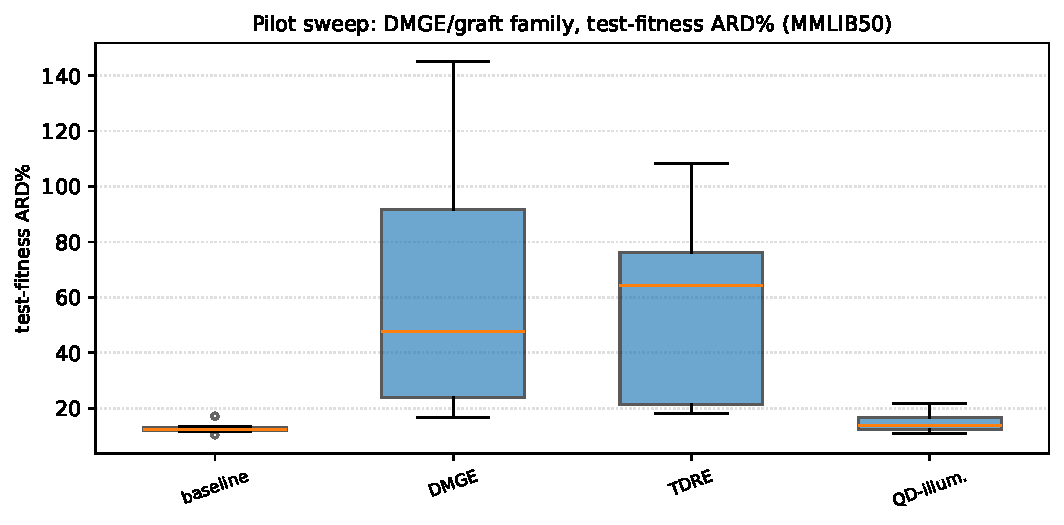
\includegraphics[width=0.85\textwidth]{img/generated/pilot_dmge_boxplot.pdf}
  \caption{Distribution of held-out test-fitness ARD\% across the three
  graft/trace-based variants and the baseline, 10 seeds per box. The two
  graft-based variants' boxes barely fit on the same axis as the
  baseline's, and their spread, not just their location, is the story:
  seed-to-seed standard deviations of 33--41 ARD\% points against the
  baseline's 1.7.}
  \label{fig:pilot-dmge-boxplot}
\end{figure}

\begin{figure}[htbp]
  \centering
  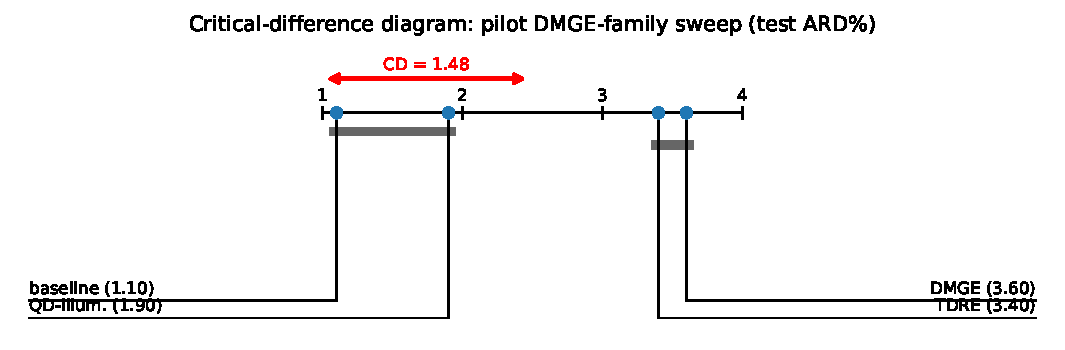
\includegraphics[width=0.85\textwidth]{img/generated/pilot_dmge_cd.pdf}
  \caption[Critical-difference diagram, pilot DMGE sweep]{Critical-difference
  diagram for the pilot DMGE-family \changed{comparison} (test ARD\%, Nemenyi CD at
  $\alpha=0.05$ for $k=4$ conditions and $N=10$ seed blocks). The baseline
  and the QD-illumination variant form one group, DMGE and TDRE a second,
  clearly separated one.}
  \label{fig:pilot-dmge-cd}
\end{figure}

The numbers in Table~\ref{tab:pilot-dmge-results}\changed{, visualised in
Figures~\ref{fig:pilot-dmge-boxplot} and~\ref{fig:pilot-dmge-cd},} turn the qualitative
verdict above into a quantitative one, and add a mechanism for the
``instability'' this section has so far described only informally. On the
common held-out test scale, DMGE and TDRE average 60.27 and 56.48 ARD\%
against the baseline's 12.74, worse in every single paired seed
($r=-1.000$), with seed-to-seed standard deviations twenty times the
baseline's; the QD-illumination variant, which grafts nothing and only
changes the archive structure, lands far closer (14.75) but still
significantly worse ($p=0.0176$). Part of the graft variants' collapse has
an identifiable cause that is itself instructive: their evolved rules lean
on the NR-dependent graft vocabulary, terminals that are only meaningful
on the NR-preserving instances they trained on and degrade to neutral
constants on the common test set, so entire grafted branches of the
evolved trees go inert at test time. A mechanism that conditions its
repairs on instance-set-specific terminals does not merely fail to help;
it produces rules that cannot survive a change of instance distribution.
An independent replication of \changed{the pilot comparison} on a disjoint seed set
reproduced this collapse in full (DMGE 38.05, TDRE 51.92 mean test ARD\%,
both still worse than the baseline in essentially every paired seed), so
the family's failure is a property of the mechanism, not of one draw of
seeds. \changed{None of the three variants justified the comprehensive
stage's cost, and none reappear in
Section~\ref{sec:operator-evaluation}.}

\changed{While DMGE did not provide the expected improvement, some of the
individual modifications were worth evaluating on their own. Modification
2's non-renewable-resource terminals are the clearest case: inside DMGE
their individual contribution could not be separated from the graft
mechanism's instability and cost. After the graft-based schemes were set
aside, these terminals were extended with a third, forward-looking one
(\texttt{NR\_BUDGET\_PRESSURE}, Section~\ref{subsec:nr-terminals-definition})
and evaluated as a strictly additive change to the terminal set, with no
grafting logic around them; they went on to become this thesis's strongest
result.}

\subsection{Exploratory investigation of enriched terminal sets}
\label{subsec:pilot-terminals}

DMGE's abandonment did not end the search for a variation- or
representation-side improvement; it redirected it. Immediately after the
pivot away from graft-based variation, three further terminal-set
extensions were tried in quick succession, each motivated directly by what
the previous one had (or had not) shown, which makes this round less a
grab-bag of ideas than a single chain of reasoning carried out in code.

\textbf{Critical-path propagation terminals.} The baseline already exposes
classic CPM dates (earliest/latest start and finish) as terminals, but
computes them once and leaves the GP tree to recombine them into anything
subtler, such as slack, itself. The first idea tried was to hand the GP a
more "ready-made" critical-path signal instead: four extra per-activity
features, computed once per instance and never recomputed during a run.
\changed{Writing $f(i) = d^{\min}_i + \max_{s \in S_i} f(s)$ for the
forward propagation score (the longest minimum-duration chain from $i$ to
the sink) and $b(i) = \min_{s \in S_i} b(s) - d^{\min}_i$ for its backward
counterpart, both normalised by the CPM makespan, the four terminals are
\begin{align*}
  \texttt{CP\_FORWARD} &= f(i), &
  \texttt{CP\_BACKWARD} &= b(i),\\
  \texttt{CP\_SLACK\_SCORE} &= b(i) - f(i), &
  \texttt{CP\_PROB} &= \frac{f_{\mathrm{raw}}(i)}{\max_{j} f_{\mathrm{raw}}(j)},
\end{align*}
the last being a criticality score relative to the most critical
activity.} At pilot scale (population 60, 25 generations, 5
MMLIB50 instances, 10 seeds), this sped up convergence noticeably (a mean
of 8.7 generations to reach the best solution, against 14.4 for the
baseline) and produced the single best individual run observed in this
round, but moved neither the mean training fitness nor the held-out test
fitness in any meaningful way \changed{(Table~\ref{tab:pilot-terminals-results})}. The diagnosis was
that one of the four new terminals is algebraically identical to the
existing LS terminal, and the other three are linear recombinations of
terminals the GP could already construct: the pilot rediscovered a shortcut
to something already reachable, not new information, which explains the
convergence-speed gain without a quality gain. This diagnosis is precisely
what motivated the next idea.

\textbf{Resource-constrained critical-path (RCCP) terminals.} If
precedence-only critical-path information was already redundant, the
natural next hypothesis was that \emph{resource-driven} criticality, which
no combination of the existing precedence-only terminals can express,
would fare better. Five terminals were added along these lines.
\changed{Let $k^{*}$ be the currently most contended (bottleneck)
renewable resource, i.e.\ the one maximising the utilisation
$u_k = 1 - \mathrm{avail}_k / R^{\rho}_k$, let $u^{*} = u_{k^{*}}$, and
let $E$ be the current eligible-activity set. The terminals are
\begin{align*}
  \texttt{RCCP\_BOTTLENECK\_UTIL} &= u^{*},\\
  \texttt{RCCP\_CANDIDATE\_CONTENTION} &=
    \frac{r^{\rho}_{jmk^{*}}}{\mathrm{avail}_{k^{*}}},\\
  \texttt{RCCP\_SLACK} &= \texttt{CP\_SLACK\_SCORE} \cdot (1 - u^{*}),\\
  \texttt{RCCP\_PRESSURE\_TREND} &=
    \frac{\sum_{i \in E} \min_{m} r^{\rho}_{imk^{*}}}{\mathrm{avail}_{k^{*}}},
\end{align*}
i.e.\ the bottleneck utilisation itself, the candidate mode's demand on
the bottleneck relative to what remains, a resource-discounted slack
score, and a forward-looking demand/remaining-supply ratio over the
currently eligible activities; the fifth,
\[
  \texttt{RCCP\_RESOURCE\_CONCENTRATION} =
  1 + \frac{\sum_{k \in \mathcal{R}^{\rho}} p_k \ln p_k}{\ln |\mathcal{R}^{\rho}|},
\]
where $p_k = r^{\rho}_{jmk} / \sum_{k'} r^{\rho}_{jmk'}$ is the share of
resource $k$ in the mode's total renewable demand, is one minus the normalised
Shannon entropy of the candidate mode's demand distribution over renewable
resource types, distinguishing a mode that draws heavily on one resource
type from one that spreads its demand thinly across several.} At
the same pilot scale (population 60, 25 generations, 5 MMLIB50 instances,
10 seeds, baseline / CP-propagation / RCCP / both combined), the result was
a second null: training fitness was statistically indistinguishable across
all four conditions \changed{(Table~\ref{tab:pilot-terminals-results})}.
Giving the GP live resource-contention information, not just
precedence information, did not translate into better trees at this scale
either\changed{, a second null result alongside
critical-path propagation}.

\textbf{Mode-interaction terminals.} A third, structurally different
hypothesis remained: rather than a \emph{budget} signal (how much of a
resource is left) or a \emph{contention} signal (who is competing for it
right now), a \emph{consequence} signal, how much choosing a given mode for
one activity narrows down the feasible mode choices left for other,
not-yet-scheduled activities sharing a resource window with it.
\changed{Three terminals implement this idea. Writing $E' = E \setminus
\{j\}$ for the other currently eligible activities and
$\mathrm{avail}_k$ for the current remaining capacity of renewable
resource $k$, and $\mathcal{K}_{jm} = \{\, k : r^{\rho}_{jmk} > 0 \,\}$
for the resource types the candidate mode actually uses. With
$\phi(i) = |\{\, m' \in \mathcal{M}_i : \exists k:\;
r^{\rho}_{im'k} > \mathrm{avail}_k - r^{\rho}_{jmk} \,\}|$ counting
neighbour $i$'s modes that committing the candidate mode would make
resource-infeasible:
\begin{align*}
  \texttt{MI\_CONSTRAINT\_TIGHTENING} &=
    \frac{1}{|E'|} \sum_{i \in E'} \frac{\phi(i)}{|\mathcal{M}_i|},\\
  \texttt{MI\_RECIPROCAL\_SCARCITY} &=
    \frac{|\{\, k \in \mathcal{K}_{jm} :
      \textstyle\sum_{i \in E'} \min_{m'} r^{\rho}_{im'k} > \mathrm{avail}_k \,\}|}
      {|\mathcal{K}_{jm}|},\\
  \texttt{MI\_ACTIVITY\_PRESSURE} &=
    \frac{1}{|\mathcal{M}_j|} \sum_{m \in \mathcal{M}_j}
    \texttt{MI\_CONSTRAINT\_TIGHTENING}(j, m),
\end{align*}
i.e.\ the average fraction of neighbours' modes the candidate mode would
make infeasible; a cheaper proxy counting
for how many of the candidate's resources the neighbours' combined
cheapest-mode demand already exceeds availability; and the first measure
averaged over the candidate activity's own modes (activity tree). These}
were the least literature-established of any extension
tried, by design: there is comparatively little precedent in the published
GPHH/RCPSP literature for a consequence-based terminal of this kind, so a
null result here was always going to be exactly as informative as a
positive one. It was, in fact, worse than null
\changed{(Table~\ref{tab:pilot-terminals-results})}: mode-interaction
terminals alone were not significant against baseline
\changed{(and the mean moved in the \emph{wrong} direction)}, and stacking
them with RCCP terminals made things actively worse, significantly so.
Combining two sets of additional
terminals compounded noise rather than information, a caution worth
carrying forward whenever new terminals are added to an already-rich
feature set.

\begin{table}[htbp]
  \centering
  \small
  \caption[Pilot results: enriched terminal sets]{\changed{Pilot results for
  the enriched-terminal-set round: mean training-fitness ARD\% (\%), 10
  seeds per condition, paired two-sided Wilcoxon $p$ against the matching
  baseline run. The two blocks are separate pilot runs, each compared
  against its own baseline.}}
  \label{tab:pilot-terminals-results}
  \begin{tabular}{lrr}
    \toprule
    \textbf{Condition} & \textbf{Train mean} & \textbf{$p$} \\
    \midrule
    Baseline                         & 12.25 & --    \\
    CP-propagation terminals         & 12.39 & 0.82  \\
    RCCP terminals                   & 12.55 & 0.46  \\
    CP-propagation + RCCP            & 12.25 & 1.00  \\
    \midrule
    Baseline (second run)            & 12.40 & --    \\
    Mode-interaction terminals       & 13.37 & 0.16  \\
    Mode-interaction + RCCP          & 14.21 & 0.04 \\
    \bottomrule
  \end{tabular}
\end{table}

Read together, this second exploratory round systematically worked through
precedence-based, resource-budget-based, resource-contention-based, and
consequence-based signals, in that order, each motivated by the previous
result's diagnosis, and none of the three terminal-set ideas tried here
justified carrying forward. Non-renewable resource terminals
(Section~\ref{subsec:nr-eval}) close a different, and as it turned out
genuinely open, information gap, visibility into non-renewable rather than
renewable resource state, which is precisely why they, and not any of the
three ideas in this subsection, were the one representation-side extension
promoted to the comprehensive stage.

\subsection{\texorpdfstring{\changed{Epsilon-lexicase selection and critical-path local search: staged evaluation}}{Epsilon-lexicase selection and critical-path local search: staged evaluation}}
\label{subsec:pilot-lexicase-iteration}

\changed{The third screened direction changed the search process rather
than the representation, combining two mechanisms. Tournament selection
was replaced by epsilon-lexicase selection (module \texttt{hybrid\_gp.py};
defined in full in Section~\ref{subsec:lexicase-definition}), motivated by
the fact that tournament selection on mean deviation collapses
per-instance scores into a single number and can converge prematurely onto
generalists, whereas lexicase treats every training instance as a separate
selection case and keeps specialists alive. On top of it, a memetic
local-search step was added (module \texttt{local\_search.py}; defined in
full in Section~\ref{subsec:localsearch-definition}) that runs a
critical-path repair, mode reassignment, precedence-respecting activity
swaps, and slack-based resource shifts, on the top $8\%$ of the population
every generation. The local search only ever overwrites an individual's
recorded fitness, never the GP tree itself, so the representation remains
exactly the baseline's (the Baldwinian design of
Section~\ref{subsec:localsearch-definition}). One supporting change was
needed: fitness evaluation (\texttt{evaluate\_heuristic} in
\texttt{gphh\_solver.py}) now also stores each individual's vector of
per-instance deviations (\texttt{case\_fitness}), which is what lexicase
selection filters on, case by case.}

\changed{This combination was evaluated in four stages of increasing scale
and cost, summarised in Tables~\ref{tab:lexicase-stages}
and~\ref{tab:lexicase-stages-consequences} and described below.}

\begin{table}[htbp]
  \centering
  \small
  \shrinktofit{%
  \caption[Escalating evidence for lexicase selection]{The four
  evidence-escalation stages of the lexicase follow-up, each on serial SGS
  against the tournament baseline (stage 1 measured the combination with
  the memetic local search; stages 2--4 measured lexicase in isolation).
  The training-fitness advantage strengthens with every escalation while
  the test-fitness effect, seemingly headed for significance at stages
  2--3, reverses at stage 4, the effect-size inflation episode discussed
  below.}
  \label{tab:lexicase-stages}
  \begin{tabular}{lll}
    \toprule
    \textbf{Stage} & \textbf{Scale} & \textbf{Outcome (lexicase vs.\ baseline)} \\
    \midrule
    1. First pass (with LS) &
    pop.\ 60, gen.\ 25, 5 inst., $n{=}10$ &
    train 11.87 vs.\ 13.48; $p{=}0.0059$, $r{=}0.93$ \\
    2. Official split &
    pop.\ 60, gen.\ 20, 10 classes, $n{=}10$ &
    \changed{train 16.58 vs.\ 18.05; $p{=}0.0098$, $r{=}0.89$; test 18.57 vs.\ 19.40; $p{=}0.109$} \\
    3. Power follow-up &
    stage 2 + 6 seeds ($n{=}16$) &
    \changed{train 16.57 vs.\ 17.91; $p{=}0.00058$, $r{=}0.90$; test 18.71 vs.\ 19.43; $p{=}0.074$, $r{=}0.543$} \\
    4. Extended follow-up &
    $n{=}31$ &
    \changed{train 16.68 vs.\ 17.60; $p{=}0.0002$, $r{=}0.72$; test 18.93 vs.\ 19.22; $p{=}0.325$, $r{=}0.209$} \\
    \bottomrule
  \end{tabular}%
  }
\end{table}

\begin{table}[htbp]
  \centering
  \small
  \shrinktofit{%
  \caption[Consequences of the lexicase iteration]{The two follow-on
  decisions the iteration produced: a gap-aware early-stopping mechanism
  built to act on the train/test asymmetry, which failed both validations
  and was retired, and the $2 \times 2$ ablation design (baseline,
  lexicase alone, local search alone, combined) that was promoted wholesale
  into the comprehensive stage rather than re-run at pilot scale.}
  \label{tab:lexicase-stages-consequences}
  \begin{tabular}{lll}
    \toprule
    \textbf{Follow-on} & \textbf{Design} & \textbf{Outcome} \\
    \midrule
    Gap-aware stopping &
    two validations, $n{=}10$ &
    n.s.\ ($p{=}0.109$ / $p{=}0.734$); retired \\
    $2 \times 2$ ablation &
    pop.\ 1\,000, gen.\ 50, $n{=}30$, full grid &
    became Chapter~\ref{chap:experiments}'s condition set \\
    \bottomrule
  \end{tabular}%
  }
\end{table}

The first pilot pass (population 60, 25 generations, 5 MMLIB50 instances,
10 seeds) combined epsilon-lexicase selection with \changed{the
critical-path local search (a hill-climbing refinement of elite
individuals' schedules, defined in
Section~\ref{subsec:localsearch-definition})} and found a large,
significant effect: mean training fitness of 11.87 against the baseline's
13.48, best-of-run 10.07 against 12.35, Wilcoxon $p=0.0059$ with a large
rank-biserial effect size ($r=0.93$). Convergence was slower under lexicase
(17.5 generations to best solution, against 12.0 for the baseline), which
is exactly what a case-by-case, diversity-preserving selection pressure
would be expected to do relative to tournament selection's tendency to
collapse onto a single strong generaliser early.

A second, larger pass moved to the official 60/20/20 train/validation/test
split on real MMLIB50, stratified down to 10 of the 108 classes because the
literal paper specification (population 1\,000, 50 generations, the full
class split) would have taken an estimated 200-plus days on the hardware
available at that stage (population 60, 20 generations, 10 seeds, both
serial and parallel SGS, three conditions: baseline, lexicase, lexicase
with local search). \changedB{The same 10-class stratification was later
retained for the comprehensive stage as well
(Section~\ref{subsec:instance-sampling}): \emph{training} on the full
108-class split was never computationally within reach at the paper's own
budget, since the training set sits inside the GP loop and its cost is
paid again for every individual in every generation. Testing carries no
such multiplier, so the rules evolved at the comprehensive stage are
additionally re-evaluated, after evolution, on the complete 108-class
held-out test set (Section~\ref{subsec:full108}).} On serial SGS, both
lexicase and the full combination significantly beat the baseline on
training fitness ($p=0.0098$ and $p=0.027$); the same comparison on
held-out test fitness landed at $p=0.109$ for lexicase, same direction, not
yet under the conventional 0.05 threshold. This pass also surfaced an
unplanned finding that turned out to matter more, at this scale, than the
selection mechanism under study: serial SGS dramatically outperformed
parallel SGS for every condition (test fitness around 18--19 versus 30--33),
a scale-of-effect difference between decoding schemes that later motivated
reporting every comprehensive-stage result broken down by SGS rather than
pooled across it (Section~\ref{sec:operator-evaluation}).

A quick power calculation on the $p=0.109$, $n=10$ result (effect size
$r=0.667$) suggested that 14--16 seeds might be enough to reach
significance, so six more seeds were added to that one comparison alone
rather than re-running the full grid. \changed{Two methodological caveats
apply to this step. First, adding observations
until a test reaches significance is a form of sequential testing without
correction, which inflates the false-positive rate; had the extension
produced $p<0.05$, that value could not have been taken at face value.
Second, the power calculation itself was built on a single small-sample
effect-size estimate. Both caveats turned out to matter, in the
conservative direction:} at $n=16$, the result moved to
$p=0.074$ ($r=0.543$), still short of significance, while training fitness,
already significant at $n=10$, became more so ($p=0.00058$)\changed{, and
extending the same comparison to $n=31$ \emph{weakened} the test-fitness
effect, to $p=0.325$ and $r=0.209$, instead of strengthening it.} The
$n=10$ estimate of $r=0.667$ had been small-sample
noise, not an early signal of a real, strengthening trend, a textbook
instance of effect-size inflation from an underpowered pilot. Training
fitness, meanwhile, stayed exactly where the larger samples had already
placed it: significant, and increasingly so ($p=0.0002$, $r=0.72$,
mean 16.68 for lexicase against 17.60 for baseline). \changed{The reading
at this scale was that lexicase selection reliably fits the training
instances better, but that advantage was not showing up as significantly
better generalisation. Partly in response to this episode, every
comprehensive-stage comparison in
Section~\ref{sec:operator-evaluation} was planned at a fixed $n=30$
decided in advance, not adaptively in response to interim $p$-values.}

\changed{Despite the $n=31$ null on test fitness, lexicase remained
interesting enough to carry into the comprehensive stage: its
training-fitness advantage was the most consistent positive signal any
screened mechanism had produced, the null covered only one decision
strategy and one decoding scheme at a reduced budget, and evaluating
lexicase added little extra cost to a comprehensive experiment whose
baseline runs had to be executed in any case. The comprehensive stage then
confirmed the train/test asymmetry across the full grid and, on MMLIB100,
found that it widens rather than resolves
(Section~\ref{subsec:lexicase-eval}).}

\changed{One design decision followed directly from this iteration: a full
$2 \times 2$ ablation, baseline, lexicase alone, local search alone, and
the two combined, became the core of the comprehensive stage's
experimental design (the conditions \texttt{baseline}, \texttt{lexicase},
\texttt{local\_search} and \texttt{hybrid} of
Chapter~\ref{chap:experiments}). The ablation was needed because every
pilot result up to the second pass had measured lexicase either in
combination with the local search or alongside it, so the two mechanisms'
individual contributions could not be separated: a gain or loss observed
for the combination could belong to either component, or to their
interaction. Running all four conditions at full statistical power is what
later made it possible to show that the combination underperforms both of
its own components (Section~\ref{subsec:final-comparison}).}

One further side-investigation grew directly out of this asymmetry and
also ended in a null result. Examining per-seed
training/validation fitness trajectories suggested that lexicase's
train/validation gap stays flat for several generations and then widens
onto a stable, higher plateau, with none of the later training-fitness
gains transferring to held-out data. A gap-onset detector was built to
catch this transition from the run's own validation trajectory (not a
hard-coded generation) and used to roll back to the best-on-validation
generation's individual, or stop the run early, once onset was detected.
Validated twice, once at a scale with no real train/test gap to catch (so
inconclusive by construction) and once against a known-gap 10-class split,
the detector correctly identified the onset generation and rolled back in
8--9 of 10 seeds, to a mean generation roughly a third to half of the full
budget, but gap-aware early stopping was never significantly better than
plain lexicase on test fitness ($p=0.109$ and $p=0.734$ in the two
validations), and the generalisation gap itself barely moved. The diagnosis was that
validation-set ``best so far'' is too noisy an estimator, at only 10--25
held-out instances, to reliably identify the generation that will actually
generalise best to a third, fully held-out set: the gap is real, but this
particular way of acting on it was not precise enough to help. This
mechanism was retired after that result and is not part of the
lexicase condition evaluated in Section~\ref{subsec:lexicase-eval}.

\changed{The methodological lesson of this iteration is that an early
effect-size estimate from a small pilot, even one that looks clean and
significant, should be treated as a hypothesis about direction, not
magnitude: a follow-up power calculation built on one such estimate can
point the wrong way once more data arrives.}

\changed{Table~\ref{tab:screening-verdicts} summarises the verdict on
every screened direction: only epsilon-lexicase selection, critical-path
local search and the non-renewable resource terminals were carried
forward into the comprehensive evaluation.}

\begin{table}[htbp]
  \centering
  \small
  \shrinktofit{%
  \caption[Screening verdicts]{\changed{Summary of the exploratory
  screening: the verdict on every screened direction and where its
  evidence is reported.}}
  \label{tab:screening-verdicts}
  \begin{tabular}{lll}
    \toprule
    \textbf{Screened direction} & \textbf{Pilot outcome} & \textbf{Decision} \\
    \midrule
    DMGE / TDRE / QD illum.    & significantly worse (Table~\ref{tab:pilot-dmge-results}) & dropped \\
    CP-prop.\ / RCCP / MI terminals & null or worse (Table~\ref{tab:pilot-terminals-results}) & dropped \\
    Epsilon-lexicase selection & consistent training-fitness wins (Table~\ref{tab:lexicase-stages}) & carried forward \\
    Critical-path local search & positive first pass with lexicase (Table~\ref{tab:lexicase-stages}) & carried forward \\
    NR resource terminals      & extracted from DMGE toolkit (Section~\ref{subsec:pilot-dmge}) & carried forward \\
    \bottomrule
  \end{tabular}%
  }
\end{table}

